\chapter{Câu hỏi ôn tập}
\ANSMCQ{
	\begin{center}
		\begin{tabular}{|m{2.8em}|m{2.8em}|m{2.8em}|m{2.8em}|m{2.8em}|m{2.8em}|m{2.8em}|m{2.8em}|m{2.8em}|m{2.8em}|}
			\hline
			1D & 2D & 3C & 4B & 5C & 6D & 7C & 8D & 9A & 10D\\
			\hline
			11C & 12B & 13D & 14A & 15C & 16C  & 17A & 18B & 19A & 20A\\
			\hline
			21C & 22A & 23B & 24D & 25B &  &  &  &  & \\
			\hline
		\end{tabular}
\end{center}}
\begin{enumerate}[label=\bfseries Câu \arabic*:]
	\item Thí nghiệm nào tạo được dao động của vật?
	\begin{mcq}
		\item Thả vật chuyển động trên mặt phẳng ngang.
		\item Thả vật chuyển động từ trên xuống.
		\item Kéo con lắc lò xo chuyển động đều.
		\item Kéo vật nặng của con lắc lò xo khỏi vị trí cân bằng rồi buông nhẹ.
	\end{mcq}
\hideall{
\textbf{Đáp án D.}
}

\item Chuyển động của vật nào dưới đây \textbf{không phải} là dao động cơ?
\begin{mcq}
	\item Chuyển động của pittong trong xilanh khi động cơ hoạt động.
	\item Chuyển động của con lắc đồng hồ gắn trong đồng hồ quả lắc.
	\item Chuyển động của chiếc lá nổi trên mặt nước khi có sóng truyền qua.
	\item Chuyển động của một vật trượt trên mặt phẳng nghiêng.
\end{mcq}
\hideall{
\textbf{Đáp án D.}
}

\item Dao động điều hòa là dao động trong đó li độ của vật
\begin{mcq}(2)
	\item là một hàm bậc nhất của thời gian.	
	\item là một hàm bậc hai của thời gian.
	\item là một hàm cosin (hay sin) của thời gian.
	\item là một hàm tan của thời gian.
\end{mcq}
\hideall{
	\textbf{Đáp án C.}
}

\item Chọn phát biểu \textbf{sai}. Một vật dao động điều hòa với phương trình $x=A\cos\left(\omega t+\varphi\right)$ thì 
\begin{mcq}(2)
	\item $A$ là biên độ dao động hay li độ cực đại.
	\item $\omega$ là tần số dao động.
	\item $\left(\omega t+\varphi\right)$ là pha dao động ở thời điểm $t$.
	\item $\varphi$ là pha dao động ban đầu.
\end{mcq}
\hideall{
	\textbf{Đáp án B.}\\
	$\omega$ là tần số góc của dao động.}

\item Chu kì dao động của chất điểm là $T$ thì tần số góc trong dao động của chất điểm là 
\begin{mcq}(4)
	\item $\dfrac{1}{T}.$
	\item $\dfrac{2\pi}{\sqrt{T}}$.
	\item $\dfrac{2\pi}{T}$.
	\item $\dfrac{1}{\sqrt{T}}$.
\end{mcq}
\hideall{
	\textbf{Đáp án C.}
}

\item Chọn phát biểu \textbf{sai}. Hệ dao động tắt dần
\begin{mcq}(2)
	\item có biên độ giảm dần theo thời gian.
	\item không phải là dao động điều hoà.
	\item có cơ năng giảm dần theo thời gian.
	\item có tần số giảm dần theo thời gian.
\end{mcq}
\hideall{
\textbf{Đáp án D.}
}

\item Hiện tượng cộng hưởng thể hiện rõ nét khi
\begin{mcq}(2)
	\item tần số lực cưỡng bức nhỏ.
	\item biên độ lực cưỡng bức nhỏ.
	\item lực cản môi trường nhỏ.
	\item tần số lực cưỡng bức lớn.
\end{mcq}
\hideall{
\textbf{Đáp án C.}
}

\item Biên độ của một dao động cưỡng bức \textbf{không} phụ thuộc vào
\begin{mcq}(2)
	\item lực cản môi trường.
	\item biên độ của ngoại lực tuần hoàn.
	\item tần số của ngoại lực tuần hoàn.
	\item pha ban đầu của ngoại lực.
\end{mcq}
\hideall{
\textbf{Đáp án D.}\\
Biên độ của dao động cưỡng bức phụ thuộc và lực cản môi trường, tần số ngoại lực cưỡng bức, biên độ của ngoại lực cưỡng bức.\\
Biên độ của dao động cưỡng bức không phụ thuộc vào pha ban đầu của ngoại lực cưỡng bức.
}

\item Theo một tiêu chuẩn kĩ thuật về hệ thống treo (giảm xóc) của xe khách, tần số dao động riêng của xe ở trạng thái đầy tải không vượt quá $\SI{2.5}{\hertz}$. Với một xe khác có khối lượng toàn tải 16 tấn thì độ cứng của hệ thống treo có giá trị lớn nhất bằng bao nhiêu mà vẫn đảm bảo tiêu chuẩn trên?
\begin{mcq}(4)
	\item $\SI{3.95E6}{\newton/\meter}$.
	\item $\SI{4.25E6}{\newton/\meter}$.
	\item $\SI{6.85E5}{\newton/\meter}$.
	\item $\SI{5.26E5}{\newton/\meter}$.
\end{mcq}
\hideall{
\textbf{Đáp án A.}\\
Tần số dao động của xe:
$$f=\dfrac{1}{2\pi}\sqrt{\dfrac{k}{m}}\le \SI{2.5}{\hertz}\Rightarrow k\le \SI{3.95E6}{\newton/\meter}.$$
}

\item Con lắc đơn chiều dài $\ell=\SI{1}{\meter}$, khối lượng vật nặng $\SI{200}{\gram}$, dao động với biên độ góc $\SI{0.15}{\radian}$ tại nơi có gia tốc trọng trường $g=\SI{10}{\meter/\second^2}$. Ở li độ góc bằng $\dfrac{2}{3}\alpha_0$, con lắc có động năng bằng
\begin{mcq}(4)
	\item $\SI{352E-4}{\joule}$.
	\item $\SI{625E-4}{\joule}$.
	\item $\SI{255E-4}{\joule}$.
	\item $\SI{125E-4}{\joule}$.
\end{mcq}
\hideall{
\textbf{Đáp án D.}\\
Động năng của con lắc ở vị trí có li độ góc $\alpha=\dfrac{2}{3}\alpha_0$:
$$W_\text{đ}=\dfrac{1}{2}mg\ell\left(\alpha^2_0-\alpha^2\right)=\SI{125E-4}{\joule}.$$
}

\item Một vật dao động điều hoà với phương trình $x=\xsi{8\cos\left(5\pi t-\dfrac{\pi}{3}\right)}{\centi\meter}$ ($t$ tính bằng giây) thì pha ban đầu của dao động là
\begin{mcq}(4)
	\item $\xsi{5\pi}{\radian}$.
	\item $\xsi{\left(10t-\dfrac{\pi}{3}\right)}{\radian}$.
	\item $\xsi{-\dfrac{\pi}{3}}{\radian}$.
	\item $\xsi{\dfrac{\pi}{3}}{\radian}$.
\end{mcq}
\hideall{
	\textbf{Đáp án C.}}

\item Một vật nặng có khối lượng $m$ đang dao động điều hoà với phương trình $x=A\cos\omega t$. Mốc thế năng ở vị trí cân bằng. Động năng của vật là
\begin{mcq}(4)
	\item $m\omega A^2$.
	\item $\dfrac{1}{2}m\omega^2\left(A^2-x^2\right)$.
	\item $m\omega^2A^2$.
	\item $\dfrac{1}{2}m\omega^2A^2$.
\end{mcq}
\hideall{
	\textbf{Đáp án B.}
}

\item Khi nói về một vật dao động điều hoà, phát biểu nào sau đây là \textbf{sai}?
\begin{mcq}
	\item Thế năng của vật biến thiên tuần hoàn theo thời gian.
	\item Động năng của vật biến thiên tuần hoàn theo thời gian.
	\item Vận tốc của vật biến thiên điều hòa theo thời gian.
	\item Cơ năng của vật biến thiên tuần hoàn theo thời gian.
\end{mcq}
\hideall{
	\textbf{Đáp án D.}\\
Vật dao động điều hoà thì cơ năng của vật bảo toàn.
}

\item Một vật dao động điều hoà có đồ thị li độ - thời gian như hình bên. Tại thời điểm
\begin{center}
	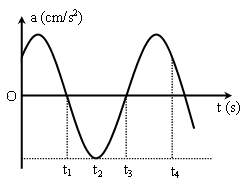
\includegraphics[width=0.4\linewidth]{../figs/C1-Q-4}
\end{center}
\begin{mcq}
	\item $t_1$ chất điểm bắt đầu chuyển động chậm dần.
	\item $t_2$ vận tốc chất điểm cực đại.
	\item $t_3$ chất điểm bắt đầu chuyển động nhanh dần.
	\item $t_4$ chất điểm có thế năng tăng.
\end{mcq}
\hideall{
\textbf{Đáp án A.}\\
Tại thời điểm $t_1$ gia tốc của chất điểm bằng 0, chất điểm chuyển động từ VTCB ra biên $\Rightarrow$ chất điểm chuyển động chậm dần.
}

\item Một vật dao động điều hoà trên trục $Ox$. Hình bên là đồ thị biểu diễn sự phụ thuộc của li độ $x$ vào thời gian $t$. Tần số $f$ của dao động là
\begin{center}
	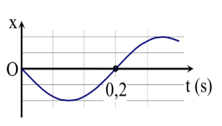
\includegraphics[width=0.3\linewidth]{../figs/C1-Q-1}
\end{center}
\begin{mcq}(4)
	\item $\SI{10}{\radian/\second}$.
	\item $\xsi{10\pi}{\radian/\second}$.
	\item $\xsi{5\pi}{\radian/\second}$.
	\item $\SI{5}{\radian/\second}$.
\end{mcq}
\hideall{
\textbf{Đáp án C.}\\
Ta có $\dfrac{T}{2}=\SI{0.2}{\second}\Rightarrow T=\SI{0.4}{\second}$.\\
Tần số góc của dao động:
$$\omega=\dfrac{2\pi}{T}=\xsi{5\pi}{\radian/\second}.$$
}

\item Đồ thị biểu diễn li độ theo thời gian của một vật dao động điều hoà được thể hiện như hình bên. Biên độ dao động là
\begin{center}
	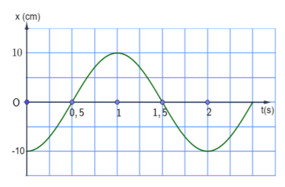
\includegraphics[width=0.4\linewidth]{../figs/C1-Q-2}
\end{center}
\begin{mcq}(4)
	\item $\SI{5}{\centi\meter}$.
	\item $\SI{-5}{\centi\meter}$.
	\item $\SI{10}{\centi\meter}.$
	\item $\SI{-10}{\centi\meter}$.
\end{mcq}
\hideall{
\textbf{Đáp án C.}
}

\item Một chất điểm dao động điều hoà, trong 10 dao động toàn phần chất điểm đi được quãng đường $\SI{120}{\centi\meter}$. Quỹ đạo của dao động có chiều dài
\begin{mcq}(4)
	\item $\SI{6}{\centi\meter}$.
	\item $\SI{12}{\centi\meter}$.
	\item $\SI{3}{\centi\meter}$.
	\item $\SI{9}{\centi\meter}$.
\end{mcq}
\hideall{
\textbf{Đáp án A.}\\
Sau mỗi chu kì dao động chất điểm đi được quãng đường $4A$, sau 10 dao động toàn phần chất điểm đi được quãng đường 
$$s=10\cdot4A=\SI{120}{\centi\meter}\Rightarrow A=\SI{3}{\centi\meter}$$
Chiều dài quỹ đạo:
$$L=2A=\SI{6}{\centi\meter}.$$
}

\item Một vật dao động điều hoà có phương trình $x=\xsi{5\cos\left(2\pi t-\dfrac{\pi}{6}\right)}{\centi\meter}$. Lấy $\pi^2=10$. Vận tốc của vật khi có li độ $x=\SI{3}{\centi\meter}$ là
\begin{mcq}(4)
	\item $v=\SI{25.12}{\centi\meter/\second}$.
	\item $v=\pm\SI{25.12}{\centi\meter/\second}$.
	\item $v=\pm\SI{12.56}{\centi\meter/\second}$.
	\item $v=\SI{12.56}{\centi\meter/\second}$.
\end{mcq}
\hideall{
\textbf{Đáp án B.}\\
Áp dụng phương trình độc lập thời gian:
$$x^2+\dfrac{v^2}{\omega^2}=A^2\Rightarrow v=\pm\omega\sqrt{A^2-x^2}=\pm\SI{25.12}{\centi\meter/\second}.$$
}

\item Một con lắc lò xo gồm lò xo có độ cứng $k=\SI{40}{\newton/\meter}$ gắn với quả cầu nhỏ. Cho quả cầu dao động với biên độ $\SI{5}{\centi\meter}$. Động năng của quả cầu ở vị trí li độ $\SI{3}{\centi\meter}$ là
\begin{mcq}(4)
	\item $\SI{0.032}{\joule}$.
	\item $\SI{320}{\joule}$.
	\item $\SI{0.018}{\joule}$.
	\item $\SI{180}{\joule}$.
\end{mcq}
\hideall{
\textbf{Đáp án A.}\\
Động năng của quả cầu ở vị trí li độ $x=\SI{3}{\centi\meter}$ là
$$W_\text{đ}=\dfrac{1}{2}k\left(A^2-x^2\right)=\SI{0.032}{\joule}.$$
}

\item Một vật dao động điều hoà có đồ thị li độ - thời gian được cho như hình bên. Lấy $\pi^2=10$. Gia tốc của vật tại thời điểm $t=\SI{1}{\second}$ là
\begin{center}
	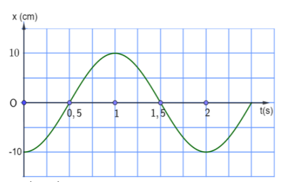
\includegraphics[width=0.4\linewidth]{../figs/C1-Q-3}
\end{center}
\begin{mcq}(4)
	\item $\SI{-100}{\centi\meter/\second^2}$.
	\item $\SI{100}{\centi\meter/\second^2}$.
	\item $\SI{-10}{\centi\meter/\second^2}$.
	\item $\SI{10}{\centi\meter/\second^2}$.
\end{mcq}
\hideall{
\textbf{Đáp án A.}\\
Chu kì dao động:
$$T=\SI{2}{\second}\Rightarrow \omega=\dfrac{2\pi}{T}=\xsi{\pi}{\radian/\second}$$
Gia tốc của vật tại thời điểm $t=\SI{1}{\second}$ là:
$$a=-\omega^2x=-\left(\xsi{\pi}{\radian/\second}\right)^2\cdot\left(\SI{10}{\centi\meter}\right)=\SI{-100}{\centi\meter/\second^2}.$$
}

\item Một vật dao động điều hoà với phương trình $x=\xsi{5\cos\pi t}{\centi\meter}$. Tốc độ trung bình của chất điểm trong khoảng thời gian bằng $\dfrac{1}{4}$ chu kì dao động kể từ lúc $t=\SI{0}{\second}$ là
\begin{mcq}(4)
	\item $\SI{1}{\centi\meter/\second}$.
	\item $\SI{2}{\centi\meter/\second}$.
	\item $\SI{10}{\centi\meter/\second}$.
	\item $\SI{20}{\centi\meter/\second}$.
\end{mcq}
\hideall{
\textbf{Đáp án C.}\\
Chu kì dao động của vật:
	$$T=\dfrac{2\pi}{\omega}=\SI{2}{\second}.$$
Tại thời điểm ban đầu vật đang ở vị trí biên dương, sau $\dfrac{1}{4}$ chu kì dao động vật đi được quãng đường $s=A=\SI{5}{\centi\meter}$. Tốc độ trung bình:
$$v_\text{tb}=\dfrac{s}{t}=\dfrac{A}{\dfrac{T}{4}}=\SI{10}{\centi\meter/\second}.$$
		}

\item Hình vẽ bên là đồ thị li độ theo thời gian của một vật dao động. Phương trình dao động của vật là
\begin{center}
	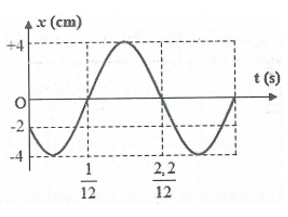
\includegraphics[width=0.4\linewidth]{../figs/C1-Q-5}
\end{center}
\begin{mcq}(2)
	\item $x=\xsi{4\cos\left(10\pi t+\dfrac{2\pi}{3}\right)}{\centi\meter}$.
	\item $x=\xsi{4\cos\left(20\pi t+\dfrac{2\pi}{3}\right)}{\centi\meter}$.
	\item $x=\xsi{4\cos\left(10\pi t+\dfrac{5\pi}{6}\right)}{\centi\meter}$.
	\item $x=\xsi{4\cos\left(20\pi t-\dfrac{\pi}{3}\right)}{\centi\meter}$.
\end{mcq}
\hideall{
\textbf{Đáp án A.}\\
Ta có:
\begin{align*}
	\begin{cases}
		A=\SI{4}{\centi\meter}\\
		\dfrac{T}{2}=\xsi{\dfrac{2,2-1}{12}}{\second}\Rightarrow T=\SI{0.2}{\second}\Rightarrow \omega=\dfrac{2\pi}{T}=\xsi{10\pi}{\radian/\second}
	\end{cases}
\end{align*}
Tại thời điểm $t=\SI{0}{\second}$ ta có 
\begin{align*}
	\begin{cases}
		x=\SI{-2}{\centi\meter}=-\dfrac{A}{2}\\
		v<0
	\end{cases}
\Rightarrow \varphi_0=\xsi{\dfrac{2\pi}{3}}{\radian}
\end{align*}
Phương trình dao động của chất điểm là $x=\xsi{4\cos\left(10\pi t+\dfrac{2\pi}{3}\right)}{\centi\meter}$.
}

\item Một con lắc dao động tắt dần trong môi trường với lực ma sát nhỏ. Cứ sau mỗi chu kì, phần năng lượng của con lắc bị mất đi $\SI{8}{\percent}$. Trong một dao động toàn phần, biên độ giảm đi
\begin{mcq}(4)
	\item $\xsi{2\sqrt{2}}{\percent}$.
	\item $\SI{4}{\percent}$.
	\item $\SI{6}{\percent}$.
	\item $\SI{1.6}{\percent}$.
\end{mcq}
\hideall{
\textbf{Đáp án B.}\\
Năng lượng còn lại sau mỗi chu kì:
$$W'=0,92W$$
Biên độ dao động còn lại sau mỗi chu kì:
$$A'=\sqrt{0,92}A=0,96A=\SI{96}{\percent}\cdot A$$
Như vậy, sau mỗi chu kì dao động biên độ của con lắc giảm đi $\SI{4}{\percent}$.
}

\item Một con lắc lò xo có độ cứng $k=\SI{100}{\newton/\meter}$ dao động điều hoà. Gọi $W_\text{t}$, $W_\text{đ}$, $W_0$ lần lượt là thế năng, động năng và cơ năng của vật năng. Đồ thị biểu diễn sự phụ thuộc của thế năng $W_\text{t}$ và động năng $W_\text{đ}$ của con lắc vào li độ như hình vẽ. Giá trị $W_0$ là
\begin{center}
	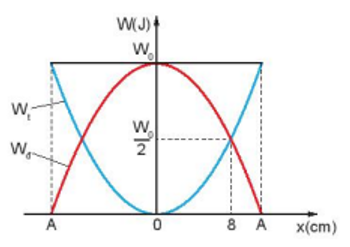
\includegraphics[width=0.4\linewidth]{../figs/C1-Q-6}
\end{center}
\begin{mcq}(4)
	\item $\SI{0.32}{\joule}$.
	\item $\SI{0.45}{\joule}$.
	\item $\SI{0.96}{\joule}$.
	\item $\SI{0.64}{\joule}$.
\end{mcq}
\hideall{
\textbf{Đáp án D.}\\
Nhận thấy khi $x=\SI{8}{\centi\meter}$ thì $W_\text{t}=\dfrac{W_0}{2}$
$$\Leftrightarrow A^2=2x^2\Rightarrow A=x\sqrt{2}=\xsi{8\sqrt{2}}{\centi\meter}$$
Cơ năng của vật nặng:
$$W_0=\dfrac{1}{2}kA^2=\SI{0.64}{\joule}.$$
}

\item Một tàu hoả chạy trên một đường ray, cứ cách khoảng $\SI{6.4}{\meter}$ trên đường ray lại có một rãnh nhỏ giữa chỗ nối các thanh ray. Chu kì dao động riêng của khung tàu trên các lò xo giảm xóc là $\SI{1.6}{\second}$. Tàu bị xóc mạnh nhất khi chạy với tốc độ bằng
\begin{mcq}(4)
	\item $\SI{10.0}{\kilo\meter/\hour}$.
	\item $\SI{14.4}{\kilo\meter/\hour}$.
	\item $\SI{16.0}{\kilo\meter/\hour}$.
	\item $\SI{20.0}{\kilo\meter/\hour}$.
\end{mcq}
\hideall{
\textbf{Đáp án B.}\\
Tàu bị xóc mạnh nhất khi thời gian vật đi hết đường ray bằng chu kì dao động riêng của khung tàu:
$$v=\dfrac{\ell}{T}=\dfrac{\SI{6.4}{\meter}}{\SI{1.6}{\second}}=\SI{4}{\meter/\second}=\SI{14.4}{\kilo\meter/\hour}.$$
}
\end{enumerate}